\begin{figure}
	\begin{center}
		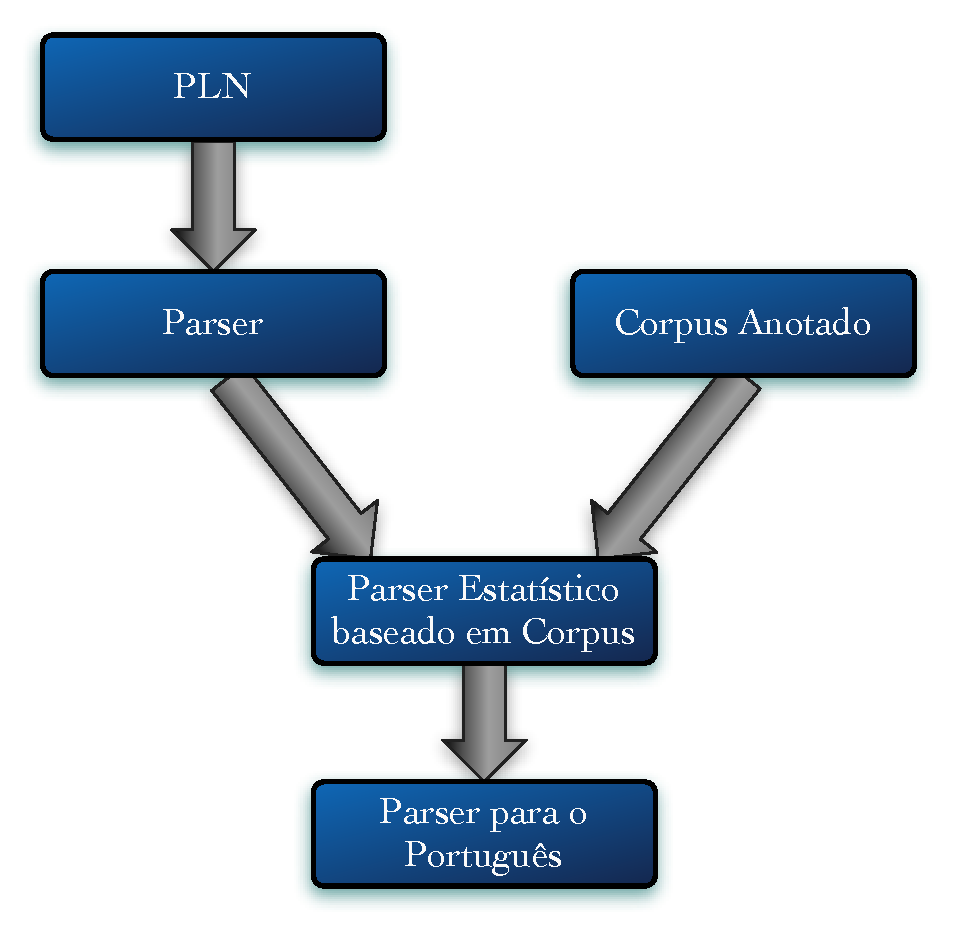
\includegraphics[scale=0.5]{fases.pdf}
		\caption{\label{fases} Insersão deste trabalho no contexto do processamento de linguagem natural propostos neste trabalho}		
	\end{center}
\end{figure}

A Figura \ref{fases} sumariza a insersão deste trabalho na área de processamento de linguagem natural. O parser desenvolvido para o português é um parser probabilístico que usa estatísticas derivadas de \emph{corpus} anotados sintaticamente para estimar os parâmetros do parser. No texto que segue abordamos alguns assuntos que fundamentam nosso trabalho.

\section{Análise de Sentença} % (fold)
\label{sec:analise_da_sentenca}

O processo de análise de sentença em linguagem natural é geralmente apresentado na literatura subdividido em vários níveis:

\begin{itemize}
	\item Análise morfológica
	\item Análise sintática
	\item Análise semântica
	\item Análise pragmática
\end{itemize}

Este trabalho foca os dois primeiros níveis de análise acima citados. Uma abordagem mais completa de todos os níveis pode ser vista em \cite{allen95,vera01} entre outros.


\subsection{Análise morfológica ou \emph{Part-of-Speech Tagging}} % (fold)
\label{sub:analise_morfologica_ou_part_of_speech_tagging}

O analisador morfológico identifica palavras ou expressões isoladas em uma sentença, sendo este processo auxiliado por delimitadores (pontuação e espaços em branco). As palavras identificadas são classificadas de acordo com seu tipo de uso ou, em linguagem natural, de acordo com sua categoria gramatical.

Neste contexto, uma instância de uma palavra em uma sentença gramaticalmente válida pode ser substituída por outra do mesmo tipo (exemplo: substantivos, pronomes, verbos, etc.), configurando uma sentença ainda válida. Para um mesmo tipo de palavra, existem grupos de regras que caracterizam o comportamento de um subconjunto de vocábulos da linguagem (exemplo: formação do plural de substantivos terminados em ``ão'', flexões dos verbos regulares terminados em ``ar'', etc.). Assim, a morfologia trata as palavras quanto à sua estrutura, forma, flexão e classificação, no que se refere a cada um dos tipos de palavras.

Esta fase é frequentemente chamada de \emph{part-of-speech tagging}, pois seu principal resultado é a determinação da categoria sintática das palavras individuais como ocorrem na sentença, também conhecida como \emph{part-of-speech} (POS). Entre essas categorias estão tipicamente as de nome (ou substantivo), verbo, preposição, etc. Outras características importantes podem ser obtidas nesta fase, como gênero (masculino ou feminino), número (singular ou plural), etc. Estas características secundárias, chamadas \emph{features} ou traços, de certa forma estendem a POS. Cada POS tem um conjunto diferenciado de \emph{features} apropriado que depende da aplicação do analisador e das concepções teóricas de quem a define. Na medida em que uma palavra é caracterizada pela sua categoria principal mais traços secundários, não é surpresa que haja uma razoável variabilidade na separação entre que características já devem estar embutidas na POS, e quais devem ser relegadas a \emph{features}. Por exemplo, algumas propostas podem selecionar como POS nome e como \emph{feature} número (singular ou plural). Outras podem atribuir POS \emph{tags} (marcações de POS) separados para nome-singular e nome-plural.

Os algoritmos para etiquetagem fundamentam-se em dois modelos mais conhecidos: os baseados em regras e os estocásticos. Os algoritmos baseados em regras, como o nome diz, fazem uso de bases de regras para identificar a categoria de um certo item lexical. Neste caso, novas regras vão sendo integradas à base à medida que novas situações de uso do item vão sendo encontradas. Os algoritmos baseados em métodos estocásticos costumam resolver as ambiguidades através de um \emph{corpus} de treino, marcado corretamente (muitas vezes através de esforço manual), calculando a probabilidade que uma certa palavra ou item lexical terá de receber uma certa etiqueta em certo contexto. O etiquetador de Eric Brill \cite{brill95}, bastante conhecido na literatura, faz uso de uma combinação desses modelos.

A escolha de um bom \emph{tagset} é fundamental para o sucesso de um \emph{parser}, embora não seja absolutamente claro como fazer este julgamento. Existem vários livros inteiros dedicados a este assunto \cite{abeille03} \cite{sardinha04}. Em linhas gerais, um bom \emph{tagset} para um \emph{parser} é aquele que possui uma boa caraterística de "equivalência distribucional" em termos sintáticos; isto é, palavras que ocorrem tipicamente nas mesmas posições nas sentenças têm mesmo POS, enquanto que as que têm características de distribuição diferentes na mesma sentença têm POS diferente. Na abordagem de Collins \cite{collins99} que usamos neste trabalho a etiquetagem é parte integrande no algorítmo de \emph{parser}.

O conjunto de tags (\emph{tagset}) utilizado nesse trabalho é definido em \cite{florestasintatica}

\subsection{Análise sintática ou \emph{Parsing}} % (fold)
\label{sub:analise_sintatica_ou_parsing}

Através da gramática da linguagem a ser analisada e das informações do analisador morfológico, o analisador sintático procura construir árvores de derivação para cada sentença, mostrando como as palavras estão relacionadas entre si.

Durante a construção da árvore de derivação, é verificada a adequação das seqüências de palavras às regras de construção impostas pela linguagem, no processo de composição das sentenças. Dentre estas regras, pode-se citar a concordância e a regência nominal e/ou verbal, bem como o posicionamento de termos na frase.

A tarefa de um \emph{parser} para a linguagem natural é construir a estrutura sintática da sentença, dividindo-a em subconstituintes de uma forma que reflita, segundo alguma teoria da linguagem, a estrutura composicional de análise da sentença. Esta estrutura é geralmente dada como uma árvore de constituintes, em que os nodos folhas são as POS, com as respectivas palavras, e os nodos internos os conhecidos como sintagmas ou categorias sintáticas de mais alto nível.

\begin{figure}
	\begin{center}
		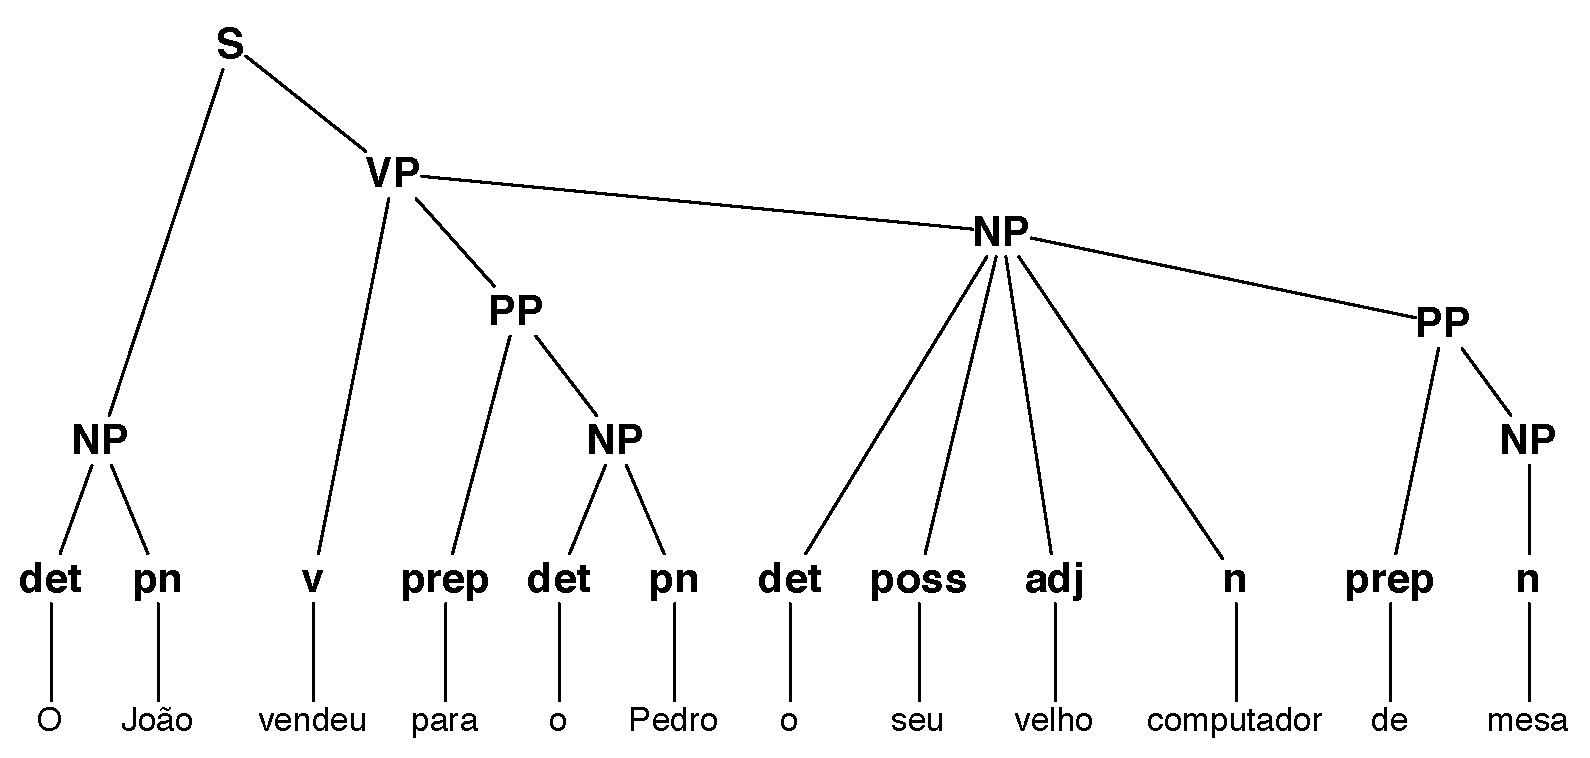
\includegraphics[scale=0.5]{tree.pdf}
		\caption{\label{tree} Árvore gramatical da frase \emph{O João vendeu para Pedro o seu velho computador de mesa}}

	\end{center}
\end{figure}

Por exemplo, a frase "O João vendeu para Pedro o seu velho computador de mesa", seria anotada gramaticalmente da seguinte forma:

\begin{verbatim}
  (S
     (NP (DET O) (PN João))
     (VP
        (V vendeu)
        (PP (PREP para) (NP (DET o) (PN Pedro)))
        (NP
            (DET o)
            (POSS seu)
            (SDJ velho)
            (N computador)
            (PP (PREP de) (NP (N mesa))))))
\end{verbatim}

			
A Figura \ref{tree} ilustra a mesma árvore em formato gráfico.

O conjunto de rótulos sintáticos utilizados nas árvores sintáticas do parser que construímos para o português esta em \cite{florestasintatica}.


% subsection análise_sintática_ou_parsing (end)

% section análise_da_sentença (end)

\section{\emph{Corpus} Anotado} % (fold)
\label{sec:corpus_anotado}

Segundo \cite{sardinha04}, \emph{corpus} é um conjunto de dados linguísticos (pertencentes ao uso oral ou escrito da língua, ou a ambos), sistematizado segundo alguns critérios, suficientemente extenso em amplitude e profundidade, de maneira que seja representativo da totalidade do uso linguístico ou de algum de seus âmbitos, disposto de tal modo que possa ser processado por computador, com a finalidade de propiciar vários, e úteis, resultados para a descrição e análise.

\emph{Corpora} anotados sintaticamente, também conhecidos como \emph{treebanks} \cite{abeille03}, são - simplificadamente - bancos de dados de sentenças anotadas com informações sintáticas e semânticas que servem como fonte de aprendizado para os sistemas estatísticos. A qualidade e o tamanho do \emph{treebank} influenciam diretamente a qualidade do resultado obtido pelo \emph{parser}. A criação do primeiro \emph{corpus} anotado data do início dos anos 60, e foi desenvolvido inicialmente para o inglês. O objetivo era prover um esquema de anotação mais completo possível, para ser utilizado por esses métodos empíricos, isto tendo em vista processamento dos corpora linguísticos. Para outras finalidades há coisas bem mais antigas

\subsection{Extensão do \emph{Corpus}} % (fold)
\label{sub:extensao_do_corpus}

A extensão e diversidade dos \emph{corpora} são definitivas na qualidade do aprendizado dos \emph{parsers} estatísticos. Conforme \cite{sardinha04}, pode-se definir três abordagens para a constituição de um \emph{corpus}.

\begin{enumerate}
\item Impressionista: baseia-se em constatações derivadas da prática da criação e da exploração de \emph{corpora}, em geral feitas por autoridades da área. Por exemplo, Aston \cite{aston97} menciona patamares que caracterizariam um \emph{corpus} pequeno (20 a 200 mil palavras) e um grande (100 milhões ou mais).

Leech \cite{leech91} fala de 1 milhão de palavras com uma taxa usual (\emph{going rate}), sugerindo o patamar mínimo. Outros são mais vagos, como Sinclair \cite{sinclair97}, que postula que o \emph{corpus} deva ser tão grande quanto a tecnologia permitir para a época, deixando subentender que a extensão de um \emph{corpus} deva variar de acordo com o padrão corrente nos grandes centros de pesquisa, que possuem equipamentos de última geração.

\item Histórica: fundamenta-se na monitoração dos \emph{corpora} eletivamente usados pela comunidade. Por exemplo, Berber Sardinha \cite{sardinha04} sugere uma classificação baseada na observação dos \emph{corpora} utilizados, segundo 4 anos de conferências de \emph{corpus}. Tabela de tamanho de \emph{corporas}:
\\




\begin{table}
   \centering
   \small
%%   \setlength{\arrayrulewidth}{2\arrayrulewidth}
%%   \setlength{\belowcaptionskip}{10pt}
   \caption{\it Tamanho de um Corpus.}

   \begin{tabular}{| c | c |}
      \hline
        \textbf{Tamanho} & \textbf{Classificação}\\
        \hline
        \hline
        Menos de 80 mil & Pequeno\\
        \hline
        80 mil a 250 mil & Pequeno-médio\\
        \hline
        250 mil a 1 milhão & Médio\\
        \hline
        1 milhão a 10 milhões & Médio-grande\\
        \hline
        10 milhões ou mais & Grande\\
        \hline

   \end{tabular}

\end{table}





\item Estatística: fundamenta-se na utilização de teorias estatísticas. Por exemplo, Biber \cite{biber93} emprega fórmulas matemáticas para identificar quantidades mínimas de palavras, gêneros e textos que se constituíram em uma amostra representativa. Algumas questões que norteiam essa abordagem são:

\begin{enumerate}
\item Dado um \emph{corpus} preexistente que serve como amostra maior, qual o tamanho mínimo de uma amostra que mantém estáveis as características da amostra maior? Essa é uma perspectiva seguida por Biber \cite{biber90,biber93}.

\item Dada uma fonte externa de referência cuja dimensão é conhecida, qual o tamanho do \emph{corpus} necessário para representar majoritariamente esta fonte? Essa vertente tem sido discutida pela comunidade de linguistas do \emph{corpus}.

\item Quanto seria perdido se o \emph{corpus} fosse de um tamanho x? Dados os recursos existentes, quais parâmetros utilizar para avalizar a decisão relativa ao tamanho de \emph{corpus} que pode ser compilado? Uma proposta segundo essa perspectiva ainda não foi formalizada, mas está presente, por exemplo, em \cite{cantossanches97.2,cantossanchez97}, que estima matematicamente a quantidade do vocabulário presente em \emph{corpora} de diversos tamanhos hipotéticos.
\end{enumerate}

\end{enumerate}

\newpage

\subsection{Corpus para processamento de linguagem natural} % (fold)
\label{sub:corpus_pln}


%%\include{vol_corpus_ingles}
\subsubsection{Corpora da Língua Inglesa}
\label{sub:corpus_ingles}

A tabela \ref{tbl:corpora} lista alguns dos corpora anotados sintaticamente mais relevantes, que são da língua inglesa.

\begin{table}
   \centering
   \small
   %%\setlength{\arrayrulewidth}{2\arrayrulewidth}
   %%\setlength{\belowcaptionskip}{10pt}
   \caption{\it Corpora da Língua Inglesa.}

   \begin{tabular}{ | p{5cm} | p{3cm} | p{3cm} | p{3cm} | }
      \hline
        \textbf{Corpus} & \textbf{Lançamento, referência na literatura} & \textbf{Palavras}& \textbf{Composição}\\
        \hline
        \hline
        Bank of English & 1987 \footnotemark[1] & 459 milhões & inglês britânico\\
        \hline
        Longman Writen American Corpus & 1997 & 100 milhões  & inglês americano, escrito ( jornais e livros )\\
        \hline
        DNC ( British National Corpus ) & 1995 & 100 milhões  & inglês britânico escrito e falado.\\
        \hline
        LLEC ( Longman-Lancaster English Language Corpus ) & 1988 & 30 milhões  & inglês de vários tipos , escrito e falado.\\
        \hline
        CHILDES (Child Language Data Exchange) & 1990 & 20 milhões & inglês infantil, falado.\\
        \hline
        The Penn TreeBank & 1989 & 10 milhões & inglês americano, escrito e falado.\\
        \hline
        Brown Corpus ( Brown University Standart Corpus of Present-day American English ) & 1964 & 1 milhão  & ingles americano, escrito\\
        \hline
   \end{tabular}
   \footnotemark[1]{Data refere-se ao Birmingham Corpus, do qual o Bank of English derivou}
   \label{tbl:corpora}
\end{table}

Existem outros corpora além dos acima elencados, que possuem um número menor de palavras. Três corpora da lista servem como marcos de referência históricos:

Brown, BNC e Bank of English. O \emph{corpus} Brown é um marco por razões óbvias: é o primeiro. O BNC é de destaque porque foi o primeiro a conter 100 milhões de palavras. Enquanto o Brown e o BNC são \emph{corpus} de amostragem, planejados e fechados, O Bank of English é um \emph{corpus} monitor, orgânico e em crescente expansão.


\subsubsection{Penn TreeBank}
\label{sub:corpus_ingles_esquema_pen}

O Penn TreeBank é um dos principais \emph{corpus} disponíveis, contem aproximadamente 7 milhões de palavras com anotação de POS, 3 milhões de palavras com ``esqueleto de parsing", mais de 2 milhões de palavras de texto anotado com informação predicado-argumento (\emph{predicate-argument structure}), e 1.6 milhões de palavras de transcrição de conversas. O material anotado possui diferentes origens e gêneros como manuais de computadores da IBM, anotações de enfermeiras, artigos do Wall Street Journal e transcrições de conversas telefônicas, entre outras.

A maioria das anotações do Penn Treebank consiste em anotação de POS, estrutura sintática e estrutura predicado-argumento dos textos escritos como os artigos do Wall Street Journal.

O conjunto de rótulos sintáticos e de POS (\emph{tagset}) usado no Penn Treebank, como muitos outros \emph{corpus}, foi baseado no Brown Corpus e é mostrado nas tabelas \ref{tbl:penn_treebank_pos} (Rótulos de Part-of-Speech) e \ref{tbl:penn_treebank_cats} (Rótulos de Categorias Sintáticas), contendo 36 tags de POS, 9 tags para pontuação e 17 tags para anotação sintática. Uma descrição detalhada do \emph{tagset} do Penn Treebank é encontrado no \emph{website} do projeto Penn Treebank em http://www.cis.upenn.edu/~treebank.

\begin{table}
   \centering
   \small
   %%\setlength{\arrayrulewidth}{2\arrayrulewidth}
   %%\setlength{\belowcaptionskip}{10pt}
   \caption{\it Rótulos de Part-of-Speech do Penn Treebank.}

   \begin{tabular}{| p{2cm} | p{4cm} | p{2cm} | p{4cm} |}

   \hline

		CC & Conjunção Coordenativa 	& 	PRP & Pronome Pessoal\\
    \hline
		CD & Numeral &   	PRP\$ & Pronome Possessivo\\
      \hline
		DT & Determinador     &		RB & Advérbio\\
      \hline
		EX & Pronome expletivo existencial ``there''     &		RBR & Advérbio, comparativo\\
      \hline
		FW & Palavra estrangeira     &		RBS & Advérbio, superlativo\\
      \hline
		IN & Preposição ou conjunção subordinada      &		RP & Partícula\\
      \hline
		JJ & Adjetivo      &		SYM & Símbolo\\
      \hline
		JJR & Adjetivo comparativo      &		TO & Qualquer ocorrência da palavra ``TO''\\
      \hline
		JJS & Adjetivo superlativo      &		UH & Interjeição\\
      \hline
		LS & Marcador de item em listas      &		VB & Verbo infinitivo\\
      \hline
		MD & Verbo auxiliar ou modal      &		VBD & Verbo passado\\
      \hline
		NN & Nome, singular      &		VBG & Verbo gerúndio ou particípio presente\\
      \hline
		NNS & Nome, plural      &		VBN & Verbo particípio passado\\
      \hline
		NP & Nome próprio singular      &		VBP & Verbo presente, exceto na terceira pessoa singular\\
      \hline
		NPS & Nome próprio plural      &		VBZ & Verbo presente, terceira pessoa singular\\
      \hline
		PDT & Predeterminador      &		WDT & Determinador interrogativo\\
      \hline
		POS & Terminador possessivo      &		WP & Pronome interrogativo\\
    \hline
     & & 	WP\$ & Pronome interrogativo possessivo\\
    \hline
     & & 	WRB & Adverbio interrogativo  \\
    \hline
     \# & Libra sinal & \$ & Caractere\$ \\
    \hline
     . & final & , & vírgula \\
    \hline
     : & dois pontos & ( & Abre parênteses \\
    \hline
     ) & Fecha parênteses & " & aspas dupla abre/fecha \\
     \hline
     ' & aspas simples & &  \\
    \hline

   \end{tabular}
   \label{tbl:penn_treebank_pos}
\end{table}


\begin{table}
   \centering
   \small
   %%\setlength{\arrayrulewidth}{2\arrayrulewidth}
   %%\setlength{\belowcaptionskip}{10pt}
   \caption{\it Rótulos de Categorias Sintáticas do Penn Treebank.}

   \begin{tabular}{ | p{2cm} | p{4cm} | p{2cm} | p{4cm} |}

   \hline
		ADJP & Sintagma Adjetivo 	& 	ADVP & Sintagma Adverbial\\
   \hline
		NP & Sintagma nominal 	& 	PP & Sintagma preposicional\\
   \hline
		S & Sintagma de clausula declarativa simples 	& 	SBAR & Sintagma de sentença subordinada\\
   \hline
		SBARQ & Sintagma de sentença interrogativa 	& 	SINV & Sintagma declarativo com inversão de sujeito\\
   \hline
		SQ & Sintagma de questão sim/não e subconstituintes de SBARQ excluindo elemento interrogativo 	& 	 VP & Sintagma verbal\\
   \hline
		WHADVP & Sintagma adverbial interrogativo 	& 	WHNP & Sintagma nominal interrogativo\\
   \hline
		WHPP & Sintagma preposicional interrogativo &    	X & Sintagma de constituinte desconhecido \\
	\hline

   \end{tabular}
   \label{tbl:penn_treebank_cats}
\end{table}

%%\include{vol_corpus_portugues}
\subsubsection{Corpora da Língua Portuguesa}
\label{sub:corpus_portugues}

Na língua portuguesa, há alguns corpora eletrônicos de destaque. A tabela \ref{tbl:corpora_port} apresenta um pequeno resumo dos \emph{corpus} existentes para o português.

\begin{table}
   \centering
   \small
   %%\setlength{\arrayrulewidth}{2\arrayrulewidth}
   %%\setlength{\belowcaptionskip}{10pt}
   \caption{\it Corpora da Língua Portuguesa.}

    \begin{tabular}{ | p{5cm} | p{3cm} | p{3cm} | p{3cm} | }
      \hline
        \textbf{Corpus} & \textbf{Palavras} & \textbf{Composição}& \textbf{Localização}\\
        \hline
        \hline

        Banco de Português &  233 milhões & português brasileiro, escrito e falado & PUC/SP \\

        \hline

        CETEMPublico ( Corpus de extração de Textos eletrônicos MCT), (Floresta Sintática, Bosque) & 220 milhões & jornal português, ``público'' & Projeto Linguateca \\

        \hline

        Corpus UNESP/Araraquara/ Usos do português & 200 milhões & português brasileiro, escrito & UNESP / Araraquara \\

        \hline

        CRPC( COrpus de referencia do português contemporâneo) & 152 milhões & português dos vários países lusófonos, com predominância da variedade européia & CLUL - Centro de lingüística da Universidade de Lisboa. \\

        \hline

        NILC & 35 milhões & português brasileiro escrito & NILC (USP, UFSCAR, UNESP Araraquara) \\
    \hline

   \end{tabular}
   \label{tbl:corpora_port}
\end{table}

\subsubsection{Floresta Sintática (Projeto Linguateca)}
\label{sub:sub_linguateca}

Um dos objetivos da Linguateca é melhorar significativamente as condições para o processamento do português, e prover recursos para pesquisa como os repositórios do Floresta Sintática , CETEMPublico e o CETEMFolha .

O CETEMPúblico (\emph{Corpus de Extractos de Textos Eletrônicos MCT/Público}) é um \emph{corpus} de aproximadamente 180 milhões de palavras em português de Portugal, criado por um projeto de processamento computacional do português após a assinatura de um protocolo entre o Ministério da Ciência e Tecnologia português (MCT) e o jornal O Público.

O CETENFolha (\emph{Corpus de Extractos de Textos Eletrônicos NILC/Folha de São Paulo}) é um \emph{corpus} de cerca de 24 milhões de palavras em português brasileiro, criado por um projeto de processamento computacional do português com base nos textos do jornal A Folha de São Paulo que fazem parte do \emph{corpus} NILC/São Carlos, compilado pelo Núcleo Interinstitucional de Lingüística Computacional (NILC).

A Floresta Sintática é um subconjunto dos corpora CETEM Público e CETEM Folha cujas sentanças foram analisadas (morfo)sintaticamente possuindo também indicação das funções sintáticas, explicitando hierarquicamente a informação relativa à estrutura de constituintes, enfim um \emph{treebank}. Foi construído como uma colaboração entre a Linguateca e o projeto VISL. Os textos foram inicialmente anotados (analisados) automaticamente pelo analisador sintático PALAVRAS (Bick 2000) e revistos manualmente por linguistas.

Atualmente, o \emph{corpus} da Floresta Sintá(c)tica tem 4 partes, que diferem quanto ao gênero textual, quanto ao modo (escrito vs falado) e quanto ao grau de revisão lingüística: o Bosque, totalmente revisto por lingüistas; a Selva, parcialmente revisto, a Floresta Virgem e a Amazônia, não revistos. Junto, todo esse material soma cerca de 261 mil frases (6.7 milhões de palavras) sintaticamente analisadas.

Para nosso estudos de desenvolvimento de um \emph{parser} probabilístico para a língua portuguesa e treino da ferramenta desenvolvida por Bikel , será utilizado o Bosque, parte da floresta sintática completamente revisada por linguistas.

O Bosque é composto por 9.368 frases, retiradas os primeiros 1000 extratos (aproximadamente) dos corpora CETENFolha e CETEMPúblico. Desde 2007, o Bosque vem passando por um novo processo de revisão, em que foram corrigidas algumas pequenas inconsistências e acrescentadas novas etiquetas. A versão final, disponível para consulta e download, é o Bosque 8.0.

Este é o \emph{corpus} mais correto da Floresta, e por isso o mais aconselhado para pesquisas em que não se prioriza tanto a quantidade, mas sim a precisão dos resultados.

Uma quantificação das etiquetas usadas no Bosque pode ser encontrada no anexo 4 da Bíblia Florestal \cite{florestasintatica}, e uma extensa documentação das opções lingüísticas tomadas durante o projeto.


\paragraph{Esquema de anotação}\label{par:corpus_bosque_esquema}\hspace*{1in}\\ \\

A Floresta Sintática foi o corpus utilizado para desenvolver o parser aqui descrito, e portanto as árvores geradas pelo parser seguem o esquema de anotação da Floresta.

Na Floresta, a cada palavra são associadas etiquetas (ou rótulos) principais (de função e de forma) e secundárias. Estas etiquetas aparecem como FUNÇÃO:forma, aonde forma corresponde ao conceito de POS. Em ``a menina gulosa", por exemplo, temos:


\begin{verbatim}
  >N:artd       a
  H:n           menina
  N<:adj        gulosa
\end{verbatim}

A anotação ``$>$N'' para a palavra ``a'' de função, e indica que a palavra em questão é dependente à esquerda (por isso o sinal ``$>$'') de um núcleo nominal (N). Já a forma de ``a'' é artigo definido. ``Menina'' é o núcleo do sintagma nominal, por isso a FUNÇÃO é H. Como a palavra em questão é um nome, a forma é n. Por fim, o adjetivo ``gulosa'' é um dependente (modificador) à direita do nome, e por isso recebe a etiqueta de FUNÇÃO (N$<$) e a etiqueta de forma adj.

A cada palavra também é associado o seu lema, e informações morfossintáticas (gênero, número, tempo, modo e pessoa para os verbos e, eventualmente, outras etiquetas indicativas de fenômenos como elipse, construções de foco etc.). As etiquetas de POS ou forma estão listadas na tabela \ref{tbl:floresta_sintatica_pos}. O rótulos sintáticos são listados na tabela \ref{tbl:floresta_sintatica_cats}.

Uma descrição detalhada do tagset da Floresta é encontrado no website do projeto Floresta Sintática em \url{http://linguateca.dei.uc.pt/Floresta/BibliaFlorestal/anexo1.html}. A versão atual do Bosque é 8.0, de 13 de Outubro de 2008, com 9.437 árvores revistas, correspondendo a 1962 extratos, 215.420 unidades e aproximadamente 183.619 palavras.

\begin{table}
   \centering
   \small
   %%\setlength{\arrayrulewidth}{2\arrayrulewidth}
   %%\setlength{\belowcaptionskip}{10pt}
   \caption{\it Tags de Part-of-Speech da Floresta Sintática.}

    \begin{tabular}{ | p{3cm} | p{10cm} |}
      \hline
        \textbf{Símbolo} & \textbf{Categoria}\\
        \hline
        \hline

    N&nome, substantivo\\
    \hline
    PROP&nome próprio\\
    \hline
    ADJ&Adjetivo\\
    \hline
    N-ADJ&flutuação entre substantivo e adjetivo\\
    \hline
    V-FIN&Verbo finito\\
    \hline
    V-INF&Infinitivo\\
    \hline
    V-PCP&Particípio passado\\
    \hline
    V-GER&Gerúndio\\
    \hline
    ART&Artigo\\
    \hline
    PRON-PERS&pronome pessoal\\
    \hline
    PRON-DET&pronome determinativo\\
    \hline
    PRON-INDP&pronome independente (com comportamento semelhante ao nome)\\
    \hline
    ADV&Advérbio\\
    \hline
    NUM&Numeral\\
    \hline
    PRP&Preposição\\
    \hline
    INTJ&Interjeição\\
    \hline
    CONJ-S&conjunção subordinativa\\
    \hline
    CONJ-C&conjunção coordenativa\\
\hline

   \end{tabular}
   \label{tbl:floresta_sintatica_pos}
\end{table}


\begin{table}
   \centering
   \small
   %%\setlength{\arrayrulewidth}{2\arrayrulewidth}
   %%\setlength{\belowcaptionskip}{10pt}
   \caption{\it Tags Sintáticos da Floresta Sintática}
   

    \begin{tabular}{ | p{3cm} | p{10cm} | }
      \hline
        \textbf{Símbolo} & \textbf{Categoria}\\
        \hline
        \hline

            NP&Sintagma nominal
            (H: nome or pronome)\\
            \hline

            ADJP&Sintagma adjetival
            (H: Adjetivo ou determinante)\\
            \hline

            ADVP&Sintagma adverbial
            (H: advérbio)\\
            \hline

            VP&Sintagma verbal
            (contém sempre MV e poderá exibir AUX)\\
            \hline

            PP&Sintagma preposicional
            (H: preposição)\\
            \hline

            CU&Sintagma evidenciador de relação de coordenação\\
            \hline

            SQ&Sequência de funções discursivas; sequência de elementos identificadores do falante, tema, etc. e do discurso propriamente dito\\


            \hline

            FCL& Oração finita\\

            \hline

            ICL&Oração infinitiva\\

            \hline

            ACL&Oração adverbial\\

            \hline


   \end{tabular}
   \label{tbl:floresta_sintatica_cats}
\end{table}


\subsubsection{Projeto Semantic Share}
\label{sub:sub_semantic_corpus}

Um objetivo principal do SemanticShare é o desenvolvimento para o português de corpora anotados da mais recente geração e da próxima geração \cite{semanticshare}, um \emph{PropBank} e um \emph{LogicalFormBank}, dos quais uma parte é paralela a bancos de dados similares que estão a ser produzidos para outros idiomas, em outros projetos.

Estes \emph{corpora} são diferentes materializações de um banco único de enunciados e correspondentes representações gramaticais. Contêm informação morfológica, sintática e semântica integradas, armazenadas internamente em HPSG \cite{branco08}, que podem ser apresentadas em uma ou mais de dentre várias visões:

\begin{enumerate}
  \item Frases
  \item Segmentos lexicais
  \item Lemas
  \item Traços de flexão
  \item Etiquetas morfossintáticas (Tabela \ref{tbl:semantic_share_cats})
  \item Entidades nomeadas e unidade multi-palavra
  \item Árvores de constituintes (Tabela \ref{tbl:semantic_share_pos})
  \item Árvores de funções e papéis semânticos
  \item Formas lógicas
\end{enumerate}

São apoiadas por ferramentas de desenvolvimento de corpora avançadas que asseguram uma extensão fácil das estruturas anotadas quando mais informação de mais dimensões lingüísticas possa ter de ser adicionada em extensões futuras (e.g. tempo, resolução de anáfora, etc), ou quando a cobertura da gramática seja aprofundada.

Estes corpora anotados representam recursos chave para o processamento do Português, incluindo:


\begin{itemize}
  \item fornecimento de uma base empírica para o estudo lingüístico deste idioma e para o desenvolvimento de ferramentas elaboradas manualmente;
  \item treinamento de ferramentas de base estatística para o processamento superficial e profundo, incluindo parsers, etiquetadores de papéis semânticos, etc;
  \item avaliação de ferramentas de processamento;
  \item  apoio à a experimentação de abordagens inovadoras em PLN multilingue, incluindo tradução automática estatística ou meta-anotação automática para a web semântica, etc...
\end{itemize}

Em um dado momento este chegou a ser o corpus escolhido para o desenvolvimento do parser. No decorrer do desenvolvimento do trabalho mudou-se para o corpus Floresta Sintática, que se encontra em estágio mais consolidado.

\paragraph{Esquema de anotação}\label{sub:semantic_anotacao}\hspace*{1in}\\

A tabela \ref{tbl:semantic_share_pos} mostra os rótulos de POS e a tabela \ref{tbl:semantic_share_cats}, os rótulos sintáticos.

\begin{table}

   \centering
   \small
   %%\setlength{\arrayrulewidth}{2\arrayrulewidth}
   %%\setlength{\belowcaptionskip}{10pt}
   \caption{\it Tags de Part-of-Speech do projeto Semantic Share.}

    \begin{tabular}{ | p{3cm} | p{10cm} | }
      \hline
        \textbf{Símbolo} & \textbf{Categoria}\\
        \hline
        \hline

    A&Adjetivo\\
    \hline
    ADV&Adverbio\\
    \hline
    C&Complementador ( que)\\
    \hline
    CARD&Cardinal\\
    \hline
    CONJ&Conjunção\\
    \hline
    D&Determinador\\
    \hline
    DEM&Pronome demonstrativo\\
    \hline
    N&Nome\\
    \hline
    P&Preposição\\
    \hline
    PNT&Símbolo de pontuação\\
    \hline
    POSS&Pronome possessivo\\
    \hline
    PPA&Particípio passado\\
    \hline
    QNT& Quantificador\\
    \hline
    V& Verbo\\
    \hline


   \end{tabular}
\label{tbl:semantic_share_pos}      
\end{table}


\begin{table}

   \centering
   \small
   %%\setlength{\arrayrulewidth}{2\arrayrulewidth}
   %%\setlength{\belowcaptionskip}{10pt}
   \caption{\it Tags sintáticos do projeto Semantic Share.}

    \begin{tabular}{ | p{3cm} | p{10cm} | }
      \hline
        \textbf{Símbolo} & \textbf{Categoria}\\
        \hline
        \hline

        ADVP& Sintagma adverbial \\
        \hline
        AP& Sintagma Adjetival\\
        \hline
        CONJP&Sintagma coordenativo\\
        \hline
        CP&Sintagma Complementizador\\
        \hline
        NP&Sintagma nominal\\
        \hline
        N'&Projeção intermediária entre N e NP\\
        \hline
        pp&Sintagma preposicional\\
        \hline
        PPA'&Projeção intermediária entre PPA e PPAP\\
        \hline
        PPAP&Sintagma de oração Passiva\\
        \hline
        S&Sintagma de sentença\\
        \hline
        SNS&Sintagma de sentença sem sujeito\\
        \hline
        VP&Sintagma verbal\\
        \hline

   \end{tabular}
   \label{tbl:semantic_share_cats}

\end{table}

Nota: Alguns sintagma são com informação de extração, por exemplo ``S/NP'' significa sintágma de sentença com extração de NP (sujeito), VP/NP significa sintágma verbal com extração de NP (objeto), e assim por diante. As ocorrências desse tipo encontradas no \emph{corpus} foram essas: S/ADVP, S/AP, S/PP, SNS/ADVP, SNS/NP, VP/ADVP, VP/AP, VP/PP.

\newpage

\section{Diagrama geral do processo de desenvolvimento de um \emph{parser} estatístico baseado em \emph{corpus}} % (fold)
\label{sec:diagrama_geral_do_processo_de_parsing_estatistico_baseado_em_corpus}

\begin{figure}
	\begin{center}
		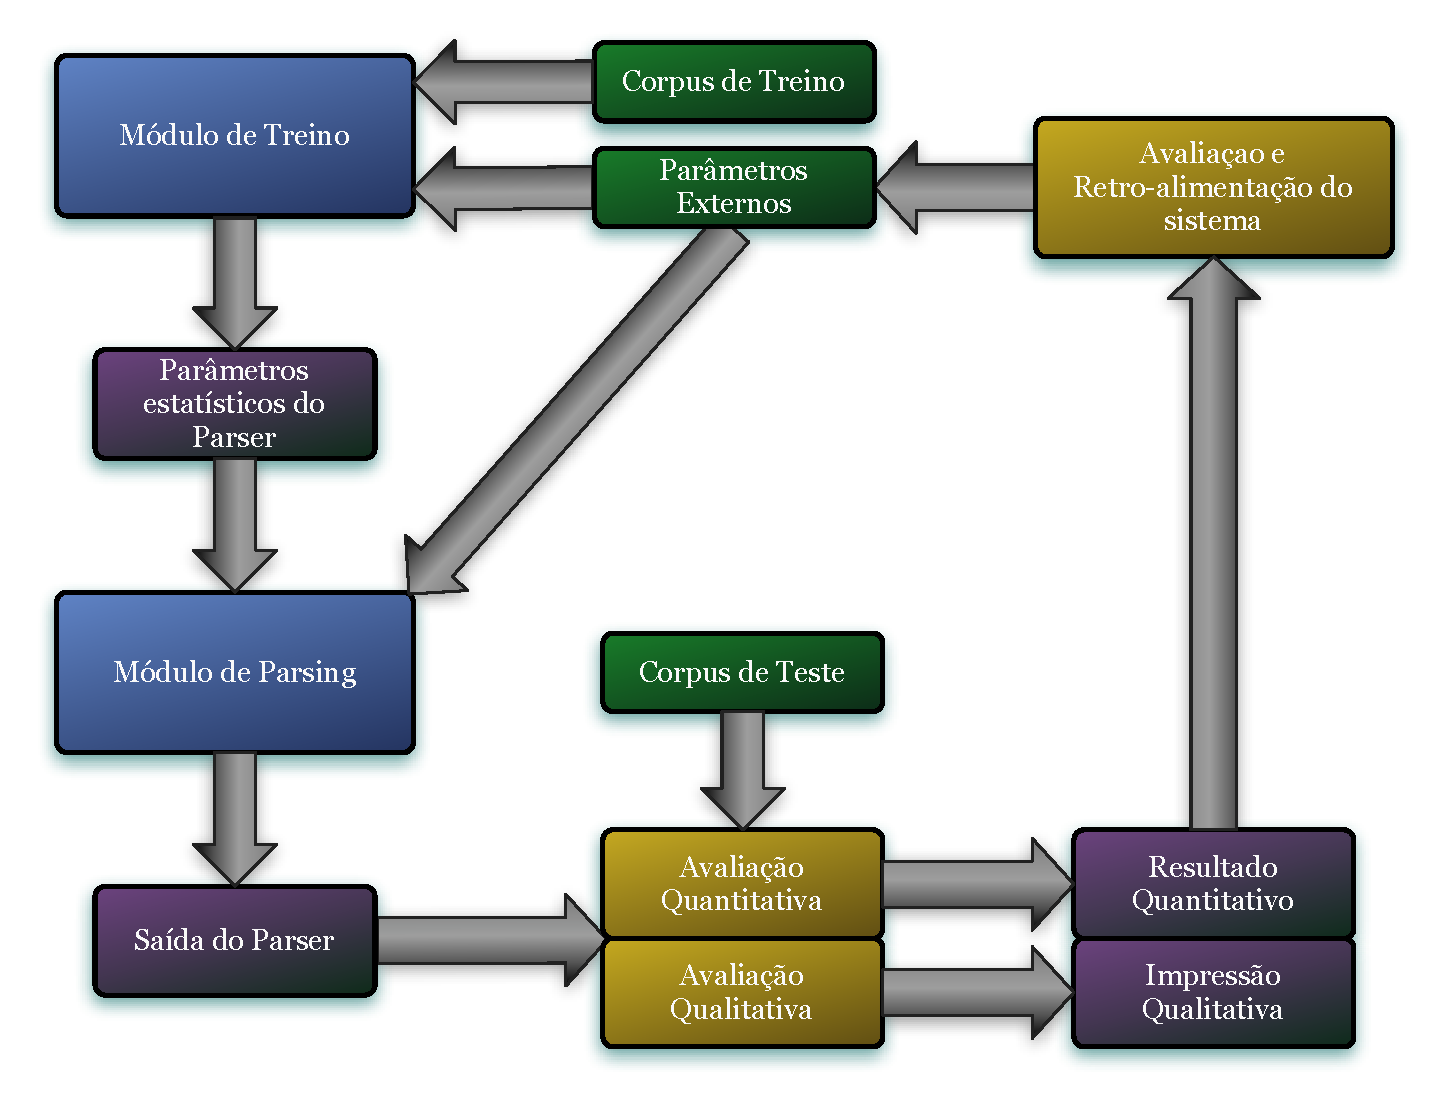
\includegraphics[scale=0.5]{parser_schema.pdf}
		\caption{\label{schema} Estágios do processamento de linguagem natural proposto pelo trabalho}		
	\end{center}
\end{figure}

Uma visão geral do processo de \emph{parsing} estatístico pode ser observada na Figura \ref{schema}. No desenvolvimento de um \emph{parser} estatístico baseado em \emph{corpus}, o \emph{corpus} anotado é dividido em 3 partes:

\begin{enumerate}

\item{Treino: Composto por sentenças que o sistema usa para aprender.} % (fold)
\label{sub:treino}

\item{Desenvolvimento (ou teste de desenvolvimento): Composto de sentenças utilizadas para avaliar a qualidade do \emph{parser} obtidas a cada passo do desenvolvimento. Como o processo de sintonia do parser é incremental e baseado em realimentação do \emph{corpus}, pode haver uma tendência de o parser ser ajustado para se adaptar ao conjunto de sentenças submetidas aos testes. Como a análise também é qualitativa, o processo de realimentação para correção do \emph{parser} tem, fatalmente, um aspecto tendencioso. Ou seja, com o tempo, o \emph{corpus} de desenvolvimento perde a isenção para representar resultados confiáveis, pois o desenvolvedor acaba adaptando o \emph{parser} para corrigir especificamente os erros feitos naquelas sentenças. 

Isto é conhecido como \emph{overfitting} \footnote{O conceito de \emph{overfitting} \cite{everitt2002cambridge} é importante na aprendizagem de máquina. Geralmente, um algoritmo de aprendizagem é treinado utilizando algum conjunto de exemplos de treinamento, ou seja, situações exemplares para que a saída desejada seja acertada. Quem aprende assume como correto o que aprendeu para também ser capaz de acertar a saída correta para outros exemplos, generalizando-se a situações não apresentados durante o treinamento (baseado em seu viés indutivo). No entanto, especialmente nos casos em que a aprendizagem foi realizada muito tempo ou quando são raros exemplos de treinamento, quem aprende pode adaptar-se a características muito específicas aleatórias dos dados de treinamento, que não têm nenhuma relação causal para a função de destino. Este processo de adaptação também ocorre com relação ao conjunto de sentenças de teste e desenvolvimento se submetidos exaustivamente à análise. Neste processo de \emph{overfitting}, o desempenho nos exemplos de formação continua a aumentar, enquanto o desempenho em conjunto de dados invisível torna-se pior.}. Para mitigar este efeito usa-se um terceiro conjunto de sentenças somente analisadas ao final do processo.} 

\label{sub:desenvolvimento_ou_teste_de_desenvolvimento_}

\item{Teste final: É semelhante ao de desenvolvimento, porém não é usado para sintonia do parser. O objetivo é que a avaliação sobre este \emph{corpus} seja insenta, sem efeito de \emph{overfitting}.}
\label{sub:teste_final}
\end{enumerate}

O módulo de geração do \emph{parser} tem como entrada os exemplos do \emph{corpus} de treino e gera os parâmetros estatísticos que serão utilizados pelo \emph{parser} para tomar as decisões. Este módulo é parametrizável com informações linguísticas fornecidas pelo desenvolvedor, que guiam a interpretação do \emph{corpus} de treino. Por exemplo, a informação de que, quando um constituinte tem dois nomes seguidos, o núcleo é o da esquerda para o português e é o da direita para o inglês.

O \emph{parser} gerado é composto pelo módulo de \emph{parsing} que recebe as sentenças de entrada e toma as decisões de análise guiado pelos parâmetros estatísticos aprendidos, gerando a sentença analisada.

Cada vez que uma nova versão (ou seja, um novo conjunto de parâmetros estatísticos) do \emph{parser} é gerada , ele é testado e os resultados do teste usados para realimentar o processo. Este teste é feito sobre o \emph{corpus} de desenvolvimento. Os resultados são analisados qualitativa e quantitativamente. Com base nestes valores, pode-se avaliar, por exemplo se a nova versão é melhor ou pior que as anteriores e o que se pode fazer para melhorar.


\section{\emph{Parsers} para Português} % (fold)
\label{sec:parsers_para_portugues}

Conforme mencionado anteriormente, existem alguns trabalhos de construção de \emph{parsers} para o português. Dentre eles, o de Eckhard Bick \cite{bick00}, baseado em regras, e portanto difícil de ser expandido ou adaptado; e os de Wing e Baldridge \cite{baldridge06} e Bonfante \cite{bonfante03}, que assim como o que aqui descrevemos são estatísticos, baseados no modelo de Collins. Entretanto, repetindo o que já mensionamos anteriormente, os resultados até agora obtidos ainda estão distantes dos desejados. A seguir descreve-se os dois trabalhos baseados em \cite{collins99}


\subsection{Trabalho de Benjamin Wing e Jason Baldridge} % (fold)
\label{sec:wing_baldridge}

Wing e Baldridge apresentaram seus resultados em \cite{baldridge06}, do desenvolvimento de um parser para o português. Assim como neste trabalho, foi utilizado como \emph{treebank} o Floresta Sintática com a ferramenta de Dan Bikel \cite{bikel02}. Foi desenvolvido um trabalho de exploração de diversos parâmetros possíveis na utilização do parser, e em termos de composição do \emph{treebank}, foram feitas alterações nas estruturas e rótulos do \emph{treebank}.

Suas métricas de desempenho utilizadas foram o PARSEVAL padrão \footnote{AS métricas do PARSEVAL para precisão e \emph{recall} de constituíntes rotulados também são descritos na seção \ref{cha:avaliacao_parceval}}, que também utilizamos nesse trabalho, e análise de dependência não rotulada. Para a análise de dependência no entanto foi necessário um trabalho \emph{ad-hoc} de tranformação do \emph{corpus} para criação de um \emph{corpus} com as relações de dependência.

Fazendo mudanças simples nos dados e na parametrização do parser de Bikel, incluindo sensibilidade morfológica ao português, mostraram sensível melhora do desempenho atingindo 63,2{\%} de \emph{F-Score} em sua melhor configuração. Em capítulo posterior reportaremos nossos resultados sensivelmente superiores a este.


\subsubsection{Preparando o material de treino, adaptações no \emph{corpus}} % (fold)
\label{sec:wing_baldridge_adapt_corpus}

Ao usar o Floresta Sintática para treino da ferramenta, Wing e Baldridge fizeram uma conversão do formato nativo para o formato PennTreebank (PTB). Para este trabalho também tivemos que fazer tal conversão uma vez que o parser de Dan Bikel espera como entrada arquivos nesse formato. Foram feitas modificações também quando a pontuação para que esta seja melhor interpretada pelo parser em formato PTB, por exemplo '.', '?' e '!' foram marcadas como '.'. 

Em principio a informação de núcleo (\emph{head}) dos sintagmas geralmente marcada explicitamente no \emph{corpus} Floresta Sintática, seria de grande ajuda no processo. O PTB não contempla essa informação. Normalmente os analisadores baseados em núcleos dos sintagmas usam regras heurísticas para inferir os núcleos durante a análise. Wing e Baldridge utilizaram-se de marcação disponível no Floresta. No entanto, como nem todos os sintágma possuem a informação de núcleo, Wing e Baldridge, ainda assim tiveram que utilizar regras heurísticas para resolver as omissões casos em que discordaram da informação constante no \emph{corpus}. Em nosso trabalhos optamos por ignorar a marcação fornecida no \emph{corpus} e parametrizar o mecanismo disponibilizado pela ferramenta de Bikel para definir o núcleo dos sintágmas.

Outra mudança feita por Wing e Baldridge no \emph{corpus} foi com relação as cláusulas conjuntivas. Cláusulas conjuntivas no Floresta são normalmente marcadas com a TAG 'CU' (\emph{Coordinating Unit})(Sintagma evidenciador de relação de coordenação), independente do tipo de constituintes coordenados. Isso faz com que no processo de treino de uma gramática, ocorram erros como confundir coordenação de sintagmas nominais com coordenações sentenciais com frequência. Neste sentido, foram alterados os labels para refletir mais especificamente as categorias dos sintágmas coordenados.

Em termos de modificação das árvores do \emph{treebank} outras transformações foram feitas, como aumentar cláusulas em NPs para distinguir cláusulas relativas das cláusulas em outras circunstâncias.

Wing e Baldridge reportaram o uso de uma série de filtros para lidar com a riqueza morfológida do português. Por exemplo: Foi usado uma lista de 39 inflexões verbais ou nominais reconhecidas par ao português, com cuidado para com falsos positivos e, ao mesmo tempo evitar a propagação de características das palavras. Deste modo temos únicos modos para lidar com varias terminações na terceira pessoa do plural do subjuntivo, mas separando 'ado' e 'ido' para evitar falsos positivo em substantivos como 'caldo' e 'Medo'. Além disso algumas terminações não são listadas como 'o' e 'a', porque elas são muito ambíguas e não são exatamente nominal ou verbal. Modificações no tratamento de plural 's' também foram necessárias pois no português quase sempre o plural é indicado por uma vogal seguida de 's', mas no ingles o plural pode ocorrer com 's' depois de várias consoantes diferentes. Este trabalho é bastante artesanal.


\subsubsection{Experimentos} % (fold)
\label{sec:wing_baldridge_experimentos}

Wing e Baldridge trabalharam com três diferentes configurações de dados e parser para experimentar o parser proposto, que variam quanto ao esforço na alteração do \emph{treebank} Floresta que foi utilizado como base.

A primeira configuração de testes leva em consideração o \emph{corpus} Floresta sem alteração e as configurações padrão da ferramenta de Bikel para o inglês. A segunda configuração leva em consideração o \emph{corpus} Floresta sem alteração mas utilizando o pacote de configuração para o português que eles construiram. O terceiro experimento utilizou o Floresta com alterações nas suas anotações e o pacote para o português.

O primeiro representa uma abordagem mais preguiçosa, ou seja não faça nada que não seja garantir que as árvores geradas possam ser analisadas pelo parser. O segundo faz o analisador de reconhecimento da linguagem, aplicando as regras definidas para o português e as configurações ajustadas. O terceiro e último experimento envolve mudar as próprias árvores do \emph{corpus} fornecendo para o parser mais informação para o processo de análise.

Para estes experimentos foi criado um conjunto de 7497 sentenças, dessas 1877 para testes e as restantes para treino.

O cálculo \emph{F-score} para o primeiro experimento foi de 38.06{\%}, para o segundo de 63.8{\%} e para o tereceiro de 67.1{\%} 

Os desempenhos com relação a configuração básica tiveram grande melhora, simplesmente inserindo o pacote de parâmetros para português ao invés de utilizar o padrão inglês, em particular, as regras de inferência do núcleo dos sintágmas. Ao se adaptar um analisador como o de Bikel par auma nova linguagem vale claramente a pena colocar um mínimo de esforço para se definir um cojunto de regras de inferência do núcleo dos sintágmas razoável (head-find rules).

\subsection{Parsing probabilístico para o português do Brasil de Andréia Gentil Bonfante} % (fold)
\label{sec:bonfante}

Bonfante em sua tese \cite{bonfante03}, faz uma investigação de métodos estatísticos quando utilizados para analisar sentenças da língua portuguesa do Brasil, implementando o método de modelo gerativo de Michael Collins \cite{collins99}. Como resultado apresenta uma ferramenta para processamento de linguagem natural, PAPO, formada por vários módulos que executam 3 funções básicas: o pré-processamento e a preparação dos dados do conjunto de sentenças usadas no treino; a geração de dois modelos probabilísticos de análise (PAPO I e PAPO II); e um \emph{parser} propriamente dito que usa um dos modelos gerados e produz as árvores sintáticas mais prováveis para uma sentença.

Nesta tese Bonfante não chegou a realizar uma avaliação abrangente e robusta de sua ferramenta, em nenhum de seus modelos. Bonfante preferiu realizar uma investigação qualitativa do desempenho do sistema, com o intuito de identificar problemas mais aparentes que surgissem na análise de um conjunto seleto de sentenças, realizando análise apenas nas sentenças consideradas mais dificeis.

Não é possível avaliar a qualidade dos resultados tanto da versao I quanto da versão II de sua ferramenta, uma vez que Bonfante usou um volume muito pequeno de casos de teste.

Em todos os experimentos realizados na tese de Bonfante, o sistema utiliza como fonte de exemplos de análise, o CENTENFolha, proveniente do Floresta Sintática.

Assim como nos trabalhos semelhantes Bonfante teve que gerar um módulo de pré-processamento para as sentenças originais, um módulo de filtro de regras, que tem como entrada as sentenças do CENTENFolha e tem como saida regras, para que possam ser usadas na geração dos modelos de sua tese.

Além do filtro de regras foi preciso criar o filtro de núcleos de sentenças, os núcleos foram identificados para cada regra. 


\subsubsection{Experimentos} % (fold)
\label{sec:bonfante_experimentos}


Para avaliar quantitativamente sua ferramenta Bonfante utilizou 23 sentenças absolutamente inéditas no sentido de não terem sido observadas no treebank utilizado para treino. Antes de serem processadas pelo seu parser de acordo com seus modelos de análise, estas sentenças foram anotadas morfossintaticamente com as TAGS do treebank.

Para cada sentença configurou-se a ferramenta para que obtivesse no máximo as dez análises mais prováveis encontradas. Caso sua ferramenta não terminasse a análise de uma sentença no prazo máximo de cinco minutos, considera-o sem solução.

Os resultados são apresentados de forma quantitativa e quanto ao tempo de processamento, para processar as 23 sentenças a ferramenta levou em média 47 segundos, seus melhores resultados quanto a precisão é de 79{\%} e \emph{recall} 75{\%}.

Não achamos que seus resultados sejam relevantes para avaliar a performace de sua ferramenta uma vez que apenas 23 sentenças de origem dúbia é um universo pequeno de casos para se avaliar uma ferramenta com tal propósito.

% section parsers_para_portugues (end)




